\documentclass[12pt,twoside]{report}

\usepackage[polish,english]{babel}
\usepackage[utf8]{inputenc}
\usepackage{polski}
\usepackage{csquotes}
\usepackage[a4paper,width=150mm,top=25mm,bottom=25mm,bindingoffset=6mm]{geometry}
\usepackage{fancyhdr}
    \pagestyle{fancy}
\usepackage{graphicx}
    \graphicspath{{images/}}
\usepackage{caption}
\usepackage{subcaption}
\usepackage[backend=biber]{biblatex}
    \addbibresource{references.bib}
\usepackage{booktabs}
\usepackage{listings}
\usepackage{cprotect}
\usepackage{refcount}
\usepackage{hyperref}
	\hypersetup{colorlinks,
			citecolor=black,
			filecolor=black,
			linkcolor=black,
			urlcolor=black
	}

\begin{document}

\begin{titlepage}
    \begin{center}
        
\includegraphics[width=0.2\textwidth]{university}

        \vspace*{1cm}
        \textbf{\uppercase{Wydział Informatyki, Elektroniki i Telekomunikacji}}

        \small
        \vspace*{0.5cm}
        \uppercase{Katedra Telekomunikacji}

        \vspace{2cm}
        \large
        \textbf{PRACA DYPLOMOWA INŻYNIERSKA}

        \vspace{2cm}
        \Large
        Communication between server-server and client-server in REST architecture

        \normalsize
        \vspace{1cm}
        Komuikacja pomiędzy serwerem-serwerem i klientem-serwerem w architekturze REST

        \small
        \vspace{2cm}
        \begin{flushleft}
            \begin{tabular}{p{5cm}l}
            Autor: & Łukasz Żarnowiecki \\
            Kierunek studiów: & Elektronika i Telekomunikacja (in English) \\
            Opiekun pracy: & Grzegorz Dobrowolski
            \end{tabular}
        \end{flushleft}

        \vfill
        Kraków, 2016

    \end{center}
\end{titlepage}

\begin{titlepage}
\noindent
Uprzedzony o odpowiedzialności karnej na podstawie art\. 115 ust\. 1 i 2 ustawy
z dnia 4 lutego 1994 r.\ o prawie autorskim i prawach pokrewnych (t.j.\ Dz.U. z
2006 r.\ Nr 90, poz.\ 631 z późn.\ zm.) : ``Kto przywłaszcza sobie autorstwo
albo wprowadza w błąd co do autorstwa całości lub części cudzego utworu albo
artystycznego wykonania, podlega grzywnie, karze ograniczenia wolności albo
pozbawienia wolności do lat 3. Tej samej karze podlega, kto rozpowszechnia bez
podania nazwiska lub pseudonimu twórcy cudzy utwór w wersji oryginalnej albo w
postaci opracowania, artystyczne wykonanie albo publicznie zniekształca taki
utwór, artystyczne wykonanie, fonogram, wideogram lub nadanie.'', a także
uprzedzony o odpowiedzialności dyscyplinarnej na podstawie art.\ 211 ust.\ 1
ustawy z dnia  27 lipca 2005 r.\ Prawo o szkolnictwie wyższym (t.j.\ Dz.\ U.\ z
2012 r.\ poz.\ 572,\ z późn.\ zm.) Za naruszenie przepisów obowiązujących w
uczelni oraz za czyny uchybiające godności studenta student ponosi
odpowiedzialność dyscyplinarną przed komisją dyscyplinarną albo przed sądem
koleżeńskim samorządu studenckiego, zwanym dalej ``sądem koleżeńskim''
oświadczam, że niniejszą pracę dyplomową wykonałem(-am) osobiście, samodzielnie
i że nie korzystałem(-am) ze źródeł innych niż wymienione w pracy.

\hspace{6cm}
\makebox[6cm][s]{\dotfill}\par
\hspace{6cm}
\makebox[6cm][c]{\small Podpis dyplomanta}
\end{titlepage}


\selectlanguage{english}
\tableofcontents
\setcounter{page}{3}

\begin{abstract}
  Many people wants to easily create REST applications, but implementing all the requirements needed for such communication takes a lot of time. Why every time developers should be starting from scratch? Why not to create a tool that will help to quickly create REST applications in new modern language?

  The idea is to create a framework which will implement REST properties in Go programming language using mountable modules that could be further extended, modified or created. This language is new on the market and its missing some simple, yet powerful ways to quickly develop RESTful applications.

  The reason for utilizing REST is the fact that most of the applications needs to handle many users. Provide security of data being transfered and the fact that it is supported by every web browser, which is the way most people uses their computers nowadays.

  Following thesis should prove that choice of the REST architecture is reasonable and justified. Chapters presents implementation of core modules that are essential for any REST based application with theoretical background and related examples.
\end{abstract}


\chapter{Goals and assumptions for the framework}
\setcounter{page}{5}
\chaptermark{Goals}
Every project needs to define its goals in advance. They should be very carefully crafted. It may sometimes take a lot of time do that, but this time will not be wasted. This is crucial from a business point of view and further implementation. Imagine a situation when an application is half-finished and goals changed so dramatically that you need to start again from the scratch. This is causing both money lose and big drop of motivation of the persons who are working to make those goals a final product. REST forces some design goals that can take off from shoulders a lot of possible mistakes in first phases of project design.

\section{Functionality and motivation to create}
Communications between nodes. What does it really mean? What is node? And why should I care.

First of all let me explain what a node really is. Think about it as a some sort of independent processing unit that can either act like a client (e.g.\ user browsing Internet) or server (either physical or virtual). Then imagine that those nodes wants to pass some messages one to another, but they are only connected through Internet and they might be far away from each other.

There are many ways to solve this problem, but there are some aspects that one should really care about.


\begin{itemize}
\item Security, you do not want someone eavesdropping you and what is more important you need to know that you speaking with the right node. Imagine a situation when someone is telling you that your mother is dying just to fish you into some dangerous situation, while this is all lie.

\item Reliability, you got something important to say, but the server is down. You are left with you car and 2000 km to pass through.

\item Performance, you do not want additional overhead, because you want to handle as much nodes as you can.
\end{itemize}

Ease of implementation and well defined API\@. There are few possibilities of employing such requirements.
\begin{itemize}
\item Distributed messaging
\item WebSockets
\item Sockets
\item REST
\end{itemize}

Let us first focus on distributed messaging. The message passing is done by different kind of sockets (e.g. Unix, TCP) and there are many software on the market that deals with all the complexity well. It really works great when you deal with communication between components that are usually called micro-services on the same or remote node. Yet there is no possibility of implementing it in user browser as our goal is to have the same communication method for clients as well as servers.

WebSockets are kind of a new technique of full-duplex communication over TCP\@. They were standardized in 2011\cite{WebSockets-wiki}, but they are mature enough for production usage proved by many big companies. Performance for long standing connection is really good and it can be easily secured. The main application is real time data acquisition like stocks price variations which is not our goal, yet this technology also full fills our requirements.

Sockets similarly to distributed messaging are not supported by web browsers. It's a little bit harder to secure this kind of linkage too, yet they prove their usefulness in server to server communication where they are broadly used.

Finally we move to REST which is a software architecture style that can be easily employed in client-server and server-server communication. The communication is usually performed over HTTP and that will be in our case.

The purpose of this work is to show how easily we can establish secure connection between multiple nodes, how we can create powerful authentication and authorization system and how to scale multiple connections with simple load balancer. Also I created simple framework written in Go for kick starting development. I tried to keep code clean with a lot of meaningful comments and high percentage of tests coverage.

The whole system contains one central server (main) with load balancer for clients and servers that the main server will connect to in order to obtain some information.

\section{Implementation environment}
For the purpose of this thesis I used Go compiler for compiling the framework to binary file as it is written in that language and popular editor Vim for editing source code files. Tests were written also in Go using testing package from standard Go library. Gorilla was used as a more advanced http router than the one in Go standard library. As a version control system for tracking source code changes I used well-know and battle-tested Git.


\chapter{Framework design}
\chaptermark{Design}
REST is the software architecture style\cite{REST-wiki}. The communication is usually carried through HTTP protocol, but this is not a requirement. REST systems expose interfaces via URIs like\label{example-URI} \verb|/user| and then to interact with this resource one can use standard HTTP verbs (GET, POST, PUT and so on), but it does not need to implement all of them. Every new attempt to interact with resources is stateless, but there is a possibility of carrying additional information (i.e.\ for authorization) through HTTP headers.

\section{Explanation of architecture}
Architecture contains main server which serves data to clients (in this case users equipped with web browsers). Then it communicate with backend servers through RESTful API to get data for clients.

In addition main server is an entity which can represent multiple servers hidden behind load balancer for scaling for high load plus one additional server for storing database and shared files via NFS\@.

\begin{figure}[!htbp]
\centering
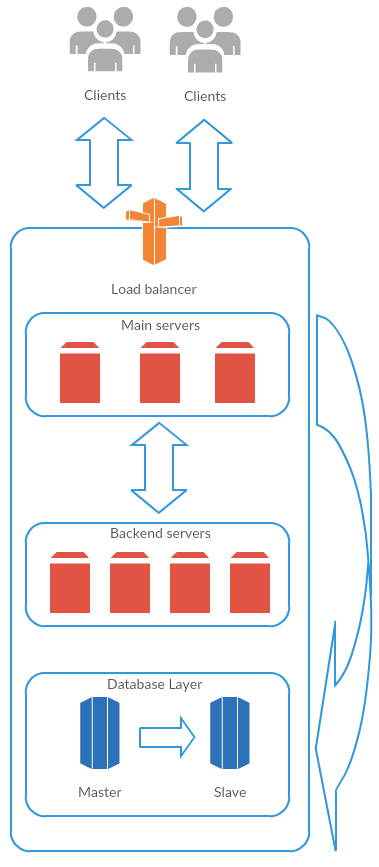
\includegraphics[scale=0.5]{architecture}
\label{fig:architecture}
\caption{Architecture of the whole system}
\end{figure}


\section{Principles}

\subsection{Uniform interface}
\label{uniform-interface}
In case of HTTP form of transporting data, every interaction can be made only through defined set of HTTP verbs as follows:

\begin{table}[!htbp]
\centering
\begin{tabular}{ll} \toprule
 HTTP verb &  Meaning \\ \midrule
 GET & Fetch resource \\
 POST & Create new resource \\
 PUT & Update resource by replacing \\
 PATCH & Update resource partially \\
 DELETE & Remove resource \\
 OPTIONS & Get list of available HTTP verbs \\ \bottomrule
\end{tabular}
\caption{HTTP verbs}
\label{tab:http-verbs}
\end{table}

Basically, in case of our example resource \verb|/user| GET, POST, PUT, PATCH, DELETE, OPTIONS would mean get user data, create new user, modify user by replacing all his data, update only few things (i.e.\ email and password), remove user, get available options (to see if I can remove user or not) respectively.

\subsection{Stateless}
\label{sec:stateless}
It means no single request depends on the previous one. By that less complexity is achieved, but as a drawback it should carry authorization information with each request (i.e.\ in HTTP headers) causing more bandwidth usage.

\subsection{Resources exposed via URIs}
\label{sec:resources}
URI\cite{URI-wiki} in short, it is a sequence of digits called string that represents specific resource. It is used commonly in WWW\@. A good example will be
\begin{verbatim}
http://google.com/a
\end{verbatim}
Breaking this up it begins with protocol name. In this case \verb|http|. Then it follows the domain name (\verb|google.com|). Those two are called URL and then after a last slash we have \verb|a| which is called URN\@. REST also tells that the URIs should be elegant, descriptive and not confusing so their meanings is straightforward.

\section{Framework design}
For the purpose of implementing aforementioned architecture a framework was created in new language ``Go'' backed by Google\cite{Go-wiki}. It can be further reused in other projects as it was released as a Free Software. The choice of Go as a language is not accidental. It has a really well defined standard library and it is very secure statically typed language with no implicit types conversions. Not to mentioned that is really fast in execution, but as a drawback writing a code feels really verbose.

Framework uses middlewares for modifying every new request and then response that is sent to a user. For instance we can create middleware purely for authentication process. If the user malformed credentials then middleware will modify the response so that the user knows that he provided them wrong.

\begin{figure}[!htbp]
\centering
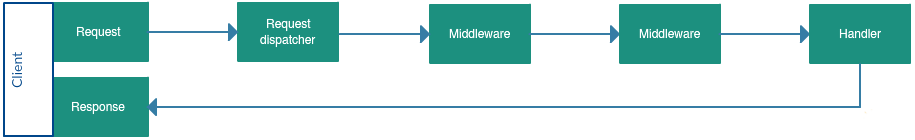
\includegraphics[scale=0.45]{middleware}
\caption[Request flow through middlewares]{Request flow through middlewares. Note that each middleware can modify request and response as they wish.}
\label{fig:middleware}
\end{figure}

\section{Authentication system and security}
Authentication system is implemented as middleware and uses standarized JWT tokens\cite{JWT-rfc}. The big benefit is that we do not need to store session in our database, we only need to verify that the token was signed by us.

The security is implemented at different levels. Connection is secured by standard TLS/SSL on HTTP level. Some resources require user to be authenticated (valid token).


\section{Strengths and weaknesses}
REST services are created from well known defined standards such as XML, JSON, URI, HTTP\@. They provide simple interfaces and they are simple to use in general. All web browsers are supporting aforementioned standards and most big websites chosen to implement RESTful services.

By it stateless nature it proves to scale well for many clients and removes complexity which has a big impact on performance and reliability.

When REST is using HTTP as a communication layer it can leverage the benefits of this protocol by using caching, clustering and load balancing which is a big win for architectures that needs to scale for millions of users.

REST was defined in 2000\cite{REST-wiki} as a style and design architecture, but being heavily tightened to HTTP it inherited all its limitations like GET can only carry 4~KB of input data\cite[p.~3]{restful-web-services}.

Another thing is performance when sending big amount of data and initializing connection every time we want to interact with resources. Unlike WebSockets, in REST we must send all the headers every time we communicate. In real time applications it is a big issue\footnote{That is the main reason behind creation of WebSockets}.

Last weakness is lack of defined security and authentication methods in standard. Therefore developers have to use TLS/SSL to secure communication and create authentication system by themselves.


\chapter{Implementation and usage of framework}
\chaptermark{Implementation}
\section{Basics}
The framework is written in Go and it contains few custom Go packages\cite{Packages-go} that can be further extended, that is
\begin{itemize}
\item \textit{common} --- contains common utilities that are used across whole framework,
\item \textit{config} --- contains package that is obliged to manage yaml based config files dependent on environmental variable,
\item \textit{middleware} --- contains middlewares, small plugins that modify requests and responses.
\end{itemize}
Every go application has a \verb|main| function which is a so called entry point and it is placed in \verb|main.go| file in the root of the project.

\section{Building}

\subsection{Prerequisities}
In order to build the project you need to have installed the following
\begin{itemize}
\item Go\footnote{\url{https://golang.org/dl}},
\item Git\footnote{\label{git-src}\url{https://git-scm.com}} (optionally).
\end{itemize}
Then you need to set up the two environmental variables
\begin{itemize}
\item GOPATH\cite[The GOPATH environment variable]{Packages-go} --- which points to your workspace directory,
\item PATH --- which should be extended by one one additional path \verb|$GOPATH/bin|
\end{itemize}

\subsection{Getting source code}
The application is stored on GitHub. In order to build it, one should fetch it at first. There are two approaches to this problem.

First, head over to website
\begin{verbatim}
github.com/Puksi-Team/RatioCare-backend
\end{verbatim}
Search for the button ``Download ZIP'' and click it. Download process will begin, after it is finished unpack it with any program of your choice\cprotect\footnote{For UNIX users issue a command \verb|unzip master.zip|.}.

Second, requires git\footnotemark[\getrefnumber{git-src}] and comes down to one command
\begin{verbatim}
go get github.com/Puksi-Team/RatioCare-backend
\end{verbatim}
which will clone the whole repository with code to your current working directory\cprotect\footnote{For UNIX users type \verb|pwd| to find out.}.

\subsection{Compiling \& Running}
To compile the project navigate to
\begin{verbatim}
$GOPATH/src/github.com/Puksi-Team/RatioCare-backend
\end{verbatim}
and issue a command \verb|go install|. It will compile and put the binary file into your \verb|$GOPATH/bin|. If you set up your PATH properly you should now be able to invoke the program just by typing its name in console.

In addition you can specify the port that the program will be listening on by \verb|-port| switch\cprotect\footnote{For more information run program with \verb|--help| switch.}.

\section{Principles of operation}

\subsection{Path of the request}
Server by default listens on port 5000. For every request the new Goroutine\cite{Goroutines-go} is being created. It is similar to thread, but basically it comes down to being a thread under the thread. Therefore every new request is handled separately and does not block the new requests. Such behaviour is provided by \textit{http}\cite{HTTP-go} package by default.

How can the application differentiate between one request or another? We need to have some sort of routing mechanism. As stated in~\ref{sec:resources} every resource is identified by URI, therefore for every URI new handler needs to be created.

For that, special type \textit{Route} was created in order to link handlers with URIs (Path) as well as HTTP method (\ref{uniform-interface}). In addition it can pass the request data by specified list of middlewares.

\begin{verbatim}
type Route struct {
        Method      string
        Path        string
        Middlewares []middleware.Middleware
        HandlerFunc http.HandlerFunc
}
\end{verbatim}

\begin{figure}[!htbp]
\begin{verbatim}
Route{
    "POST",
    "/register",
    Middlewares{
        middleware.AuthWithJwt,
        middleware.BodyParser(user.User{}),
    },
    user.RegisterHandler,
}
\end{verbatim}
\caption{Example route}
\label{src:example-route}
\end{figure}

When new request arrives the requested resource is searched linearly in array consisting all \textit{Route} definitions. When it is not found then 404 Not Found status error code is sent. Then it is client job to handle that properly. When it is found, then the request object is piped to first default middleware. Those are mandatory, like setting proper response headers, next through middlewares specified in Route object. After last middleware being finished the handler is going to be executed. In handler one can set status code, body of a response like JSON object, fetch data from database and so on.

\subsection{Building custom middleware}
Function that can be treated as a middleware must accept \verb|http.Handler| usually named \verb|next| as a parameter and return \verb|http.Handler| as well. To create a \verb|http.Handler| use \verb|http.HandlerFunc| which is an adapter\cite{HTTP-go} defined as:
\begin{verbatim}
    type HandlerFunc func(ResponseWriter, *Request)
\end{verbatim}

Now you can see that you also need to create an ordinary function with\\ \verb|ResponseWriter| and \verb|*Request| parameters where you can modify those and after you finished you should call \verb|ServeHTTP| method on \verb|http.Handler| in order to pass execution context to the next middleware or a handler. If you will not do this the response and request will never reach the handler and the client will never see a response. This function is usually defined inside function middleware as anonymous function, but it does not have to.

\begin{figure}[!htbp]
\begin{verbatim}
func SetJSONHeader(next http.Handler) http.Handler {
        handler := func(w http.ResponseWriter, r *http.Request) {
                w.Header().Set("Content-Type",
                    "application/json;charset=utf-8")
                next.ServeHTTP(w, r)
        }

        return http.HandlerFunc(handler)
}
\end{verbatim}
\caption{Example middleware that sets response headers}
\label{src:example-middleware}
\end{figure}

\subsection{Creating handler}
Handler is the last function that will be executed in execution chain\ref{fig:middleware} after all middlewares completed. The word ``Handler'' is suffixed to a function name in order differentiate between other functions.

It accepts two parameters, first \verb|http.ResponseWriter| and \verb|*http.Request|. Request object contains \verb|Method|, \verb|URL| of resource, \verb|Body|. Those are the most important and often used. When you are finished with creating response, write it to a \verb|ResponseWriter| using \verb|fmt.Fprintf| or anything else that can write to \verb|io.Writer| interface.

\subsection{Authentication mechanism}
As stated in (\ref{sec:stateless}) every request needs to carry authentication data. This kind of data is usually called token. It can be randomly generated and then saved in database. Then request token is compared with the one saved in database. In case they are different the user is not authenticated or malformed token. Otherwise we assume the request was authenticated.

But there is a better approach. Instead of storing every token in database (which is harder to test, it requires mocking database or having a running instance). We can sign the string and then verify the signature of incoming request token.

\subsubsection{Principle of operation}
Let us say the client wants to register on our website and the backend is RESTful. First he needs to make a POST request to defined resource (i.e. \verb|/register|) with required data such as an email and a password. We validate those in handler and if the data is correct token will be sent to the user in response.

The client saves the token and attaches it to every request so we can be sure that he is the person who claims to be.

\subsubsection{Token demystified}
How the token looks like? It is a string contains three parts separated by ``.'' character\cite{JWT-introduction}. Those parts represents
\begin{itemize}
\item Header,
\item Payload,
\item Signature
\end{itemize}

Header, typically contains type of token and hashing algorithm. Then it is encoded by Base64Url algorithm.
\begin{figure}[!htbp]
\begin{verbatim}
{
  "alg": "HS256",
  "typ": "JWT"
}
\end{verbatim}
\caption{Typical header of JWT token}
\label{src:typical-header}
\end{figure}

Payload, contains so called claims. Those contains data about entity (usually the user) and additional metadata. There are three types of claims
\begin{itemize}
\item Registered names, those are reserved and defined by RFC standard. They can contain information like expiration date of the token\cite{JWT-rfc},
\item Public names, they can be defined by the user, like email address, set of privileges, but the creator is responsible for creating namespace to avoid collisions,
\item Private names, created to share information that both parties agree on using them.
\end{itemize}
Then encode that with Base64Url algorithm.

To create signature, take the encoded header, encoded payload. Concatenate them with ``.'' and use secret\footnote{It is randomly generated string only known to you} to sign that with algorithm of your choice. Then it is used to verify the authenticity of the token and validate data (header and payload).

\begin{figure}[!htbp]
\begin{verbatim}
HMACSHA256(
  base64UrlEncode(header) + "." +
  base64UrlEncode(payload),
  secret)
\end{verbatim}
\caption{Pseudocode that generates signature from header and payload}
\label{src:signature}
\end{figure}



\chapter{Testing of framework}
\chaptermark{Testing}
Every piece of software should be written in a way that is testable. Moreover it is really important for framework to have tests. There are many ways to test software. Two main categories emerged when dealing with this problem. Manual, which comes down to compile, run and observe behaviour and if it matches your expectations then proceed with testing of another functionality. Automatic, there are many approaches here. The one that was performed for the purpose of this work is called ``unit testing''.

\section{Unit testing}
Which is also called testing in separation. What does it really mean is the fact that we only check the correctness of logic of only one particular function. Those should have at least $2^n$ unit tests where $n$ is number of branches in function body (e.g.\ ifs blocks). Every dependencies and calls to others functions have to be ``mocked''. Mocking is a technique of injecting exactly the same signature of mocked function, yet with predefined behaviour like fixed return value.

Unit testing is also specific to language of written application. In Go there is a special package \verb|testing| which provides methods to mark tests as failed.

Every file which contains unit tests must be suffixed with \verb|_test| in file name\cite{Testing-go} in order for command \verb|go test| to be able to discover where unit tests are. In addition every function must be prefixed with \verb|Test| keyword and have one argument \verb|*testing T|, because aforementioned tool for executing test will call every test function with that argument.

In body of unit test function we check the behaviour of function by calling it and comparing with expected result. Therefore it is a common pattern to called those variables ``actual'' and ``expected'. If those two are not the same then we will call method \verb|Error| or similar on \verb|*testing T| to mark the test as failed.

Go standard library defines also very handy package \verb|httptest|\cite{httptest-go} that have exactly the same signatures and interfaces as a package \verb|http|, yet no actual data is being send over http protocol, but the actual calls could be further inspected which is crucial in order to maintain logic separation.

Recall simple middleware (\ref{src:example-middleware}) for setting \verb|Content-Type| to JSON\@. The expected value of  \verb|Content-Type| is stored in \verb|expected| variable. Then we manually set up wrong header, then recorder is being created. \verb|HTTPHandlerMock| has the same interface as \verb|HTTPHandler| so it can be used as mock. Tested function is then called with mocked arguments, \verb|ServeHTTP| will spin up the faked server. Variable \verb|header| represents the actual data that is further compared to expected value. If condition is not met then message from method \verb|Errorf| will be printed to the console and command \verb|go test| will exit with non-zero status code.

\begin{figure}[!htbp]
\begin{verbatim}
func TestSetJSONHeader(t *testing.T) {
        expected := "application/json; charset=utf-8"

        r, _ := http.NewRequest("GET", "", nil)
        r.Header.Set("Content-Type", "application/x-www-form-urlencoded")

        w := httptest.NewRecorder()

        mock := &HTTPHandlerMock{w, r}
        handler := SetJSONHeader(mock)

        handler.ServeHTTP(mock.w, r)

        header := mock.w.Header().Get("Content-Type")
        if header != expected {
                t.Errorf("Expected %s, got `%s`", expected, header)
        }
}
\end{verbatim}
\renewcommand\figurename{Code}
\caption{Unit test of example middleware that sets response headers}
\label{src:test-example-middleware}
\end{figure}


\chapter{Conclusion}
The goal of this work was to implement REST framework for faster development of applications (mainly web) in modern language, in order to drastically decrease development time, and growing complexity and by taking the responsibility of some design decisions. By moving the burden of creating popular modules for setting proper headers, authentication mechanism and so on, development o web application based on this framework is much easier and less time consuming comparing to starting every time from scratch which multiplies by the number of projects created.

Architecture was designed in a such a way that encourages developers to create new plugins for some more specific tasks. Further development of this framework can bring new ones by the means of not breaking the existing functionality which is an important factor for long-lived applications. Current API and model is considered stable. The breakage might be introduced only by a new major versions.

Framework was extensively tested in a production application where it proves itself as a trusted, stable and well performed solution that scales for many users. The applications that was created based on this work is used for exchanging photos between clients and photographers, so pictures can be printed on a paper and send back to the clients. There is a lot of traffic involved during upload of those photos, yet it scales very well. Both mobile (Android) and web application consumes resources exposed by the created framework. By no means it should be very secure so no leakage of private photos will be possible.

Example architecture for testing environment was proposed in order to leverage communication between clients and servers of the main, central server. It can be further modified by adding new servers or providing additional layers depends on needs. The REST prove itself in this scenario as fast and reliable method of communication.

Framework was created in Go for everyone to use free of charge. Anyone can extend it by writing new custom middlewares or contribute to core of it. Most important code fragments were described. This also demonstrates how is easy is to create simple communication mechanism implemented in fairly new language with well designed standard library.

During the work, author of this project struggled a lot with unit testing, but finally he made it through. After the hassle, simple and beautiful framework emerged and all the requirements and expectations have been met.


\printbibliography\

\end{document}
